%%%%%%%%%%%%%%%%%%%%%%%%%%%%%%%%%%%%%%%%%
% Dreuw & Deselaer's Poster
% LaTeX Template
% Version 1.0 (11/04/13)
%
% Created by:
% Philippe Dreuw and Thomas Deselaers
% http://www-i6.informatik.rwth-aachen.de/~dreuw/latexbeamerposter.php
%
% This template has been downloaded from:
% http://www.LaTeXTemplates.com
%
% License:
% CC BY-NC-SA 3.0 (http://creativecommons.org/licenses/by-nc-sa/3.0/)
%
%%%%%%%%%%%%%%%%%%%%%%%%%%%%%%%%%%%%%%%%%

%----------------------------------------------------------------------------------------
%	PACKAGES AND OTHER DOCUMENT CONFIGURATIONS
%----------------------------------------------------------------------------------------

\documentclass[final,hyperref={pdfpagelabels=false}]{beamer}

\usepackage[orientation=portrait,size=a0,scale=1.05]{beamerposter} % Use the beamerposter package for laying out the poster with a portrait orientation and an a0 paper size

\usetheme{I6pd2} % Use the I6pd2 theme supplied with this template

\usepackage[english]{babel} % English language/hyphenation

\usepackage{amsmath,amsthm,amssymb,latexsym} % For including math equations, theorems, symbols, etc

%\usepackage{times}\usefonttheme{professionalfonts}  % Uncomment to use Times as the main font
%\usefonttheme[onlymath]{serif} % Uncomment to use a Serif font within math environments

\usepackage{graphicx}

\boldmath % Use bold for everything within the math environment

\usepackage{booktabs} % Top and bottom rules for tables

\graphicspath{{figures/}} % Location of the graphics files

\usecaptiontemplate{\small\structure{\insertcaptionname~\insertcaptionnumber: }\insertcaption} % A fix for figure numbering

%----------------------------------------------------------------------------------------
%	TITLE SECTION 
%----------------------------------------------------------------------------------------

\title{\huge Robust Virtual Scan for Obstacle Detection in Urban Environments} % Poster title

\author{He Mengwen$^{1,3}$, Eijiro Takeuchi$^{1}$, Yoshiki Ninomiy$^{2,3}$, and Shinpei Kato$^{1,3}$} % Author(s)

\institute{$^1$Graduate School of Information Science, Nagoya University\\
	$^2$Institute of Innovation for Future Society (MIRAI), Nagoya University\\
	$^3$JST/COI, Nagoya} % Institution(s)

%----------------------------------------------------------------------------------------
%	FOOTER TEXT
%----------------------------------------------------------------------------------------

\newcommand{\leftfoot}{http://www.coi.nagoya-u.ac.jp/} % Left footer text

\newcommand{\rightfoot}{alexanderhmw@gmail.com} % Right footer text

%----------------------------------------------------------------------------------------

\begin{document}

\addtobeamertemplate{block end}{}{\vspace*{2ex}} % White space under blocks

\begin{frame}[t] % The whole poster is enclosed in one beamer frame

\begin{columns}[t] % The whole poster consists of two major columns, each of which can be subdivided further with another \begin{columns} block - the [t] argument aligns each column's content to the top

\begin{column}{.02\textwidth}\end{column} % Empty spacer column

\begin{column}{0.47\textwidth} % The first column

%----------------------------------------------------------------------------------------
%	OBJECTIVES
%----------------------------------------------------------------------------------------

\begin{block}{Objectives}

\begin{itemize}
\item Develop a robust and real-time algorithm to transfer the point-cloud captured by a 3D LiDAR (e.g. Velodyne) to a 2D virtual scan (VScan) to represent the obstacles around the ego-vehicle. (Fig. \ref{fig:vscan})
\item Handle the inefficiency of general VScan methods on conditions of sloped roads (e.g. steep ramps), small objects (e.g. road curb), and overhung obstacles (e.g. barrier gate). (Fig. \ref{fig:challenge})
\end{itemize}

\begin{figure}
	\centering
	\includegraphics[width=\textwidth]{vscan}
	\caption{Transfer the 3D point-cloud to a 2D virtual scan. The word "virtual" means that the scan is not from a real 2D LiDAR but from the input 3D point-cloud; therefore, we can find an undetected area in this figure, which is a dead zone for our vehicle-borne Velodyne.}
	\label{fig:vscan}
\end{figure}

\begin{figure}
	\centering
	\includegraphics[width=\textwidth]{challenge}
	\caption{Challenging scenarios for general VScan methods. The road surface of steep ramp would be falsely detected as an obstacle; The road curb and barrier gate would be ignored as free space.}
	\label{fig:challenge}
\end{figure}

\end{block}

%----------------------------------------------------------------------------------------
%	INTRODUCTION
%----------------------------------------------------------------------------------------
            
\begin{block}{Introduction}

\begin{itemize}
\item Many intelligent vehicles rely on LiDARs for obstacle detection as well as localization and mapping.
\item The 3D LiDAR, e.g. Velodyne, can fully scan the real world at 10 Hz producing nearly 100,000 points per frame; however, directly processing a frame of point-cloud is always time-consuming.
\item The 2D LiDAR, e.g. SICK or Hokuyo, can horizontally scan the surrounding and briefly represent the obstacles as an array of range values; however, it may falsely detect sloped road surfaces as obstacles, and it cannot properly detect low or overhung obstacles.
\item The VScan is also an array of range values from a 2D compact transformation of point-cloud. Meanwhile, we developed a robust and real-time VScan algorithm to handle the sloped road, low objects and overhung obstacles. Therefore, the VScan is suitable for rapid further processing in a complex urban environment.
\end{itemize}

\end{block}

\begin{block}{Contributions}

\begin{itemize}
	\item A new data structure called \textit{Basic VScan Matrix} (BVSM) represents point-cloud around the ego-vehicle.
	\item A \textit{Simultaneous Road Filtering and Obstacle Detection} algorithm works on top of BVSM for robust VScan generation.
	\item A \textit{Sorted Array based Acceleration Method} enables real-time VScan generation.
\end{itemize}

\end{block}

%----------------------------------------------------------------------------------------
%	METHODS
%----------------------------------------------------------------------------------------

\begin{block}{Method Description}

\begin{columns}
	\begin{column}{0.4\textwidth}
		\begin{figure}
			\centering
			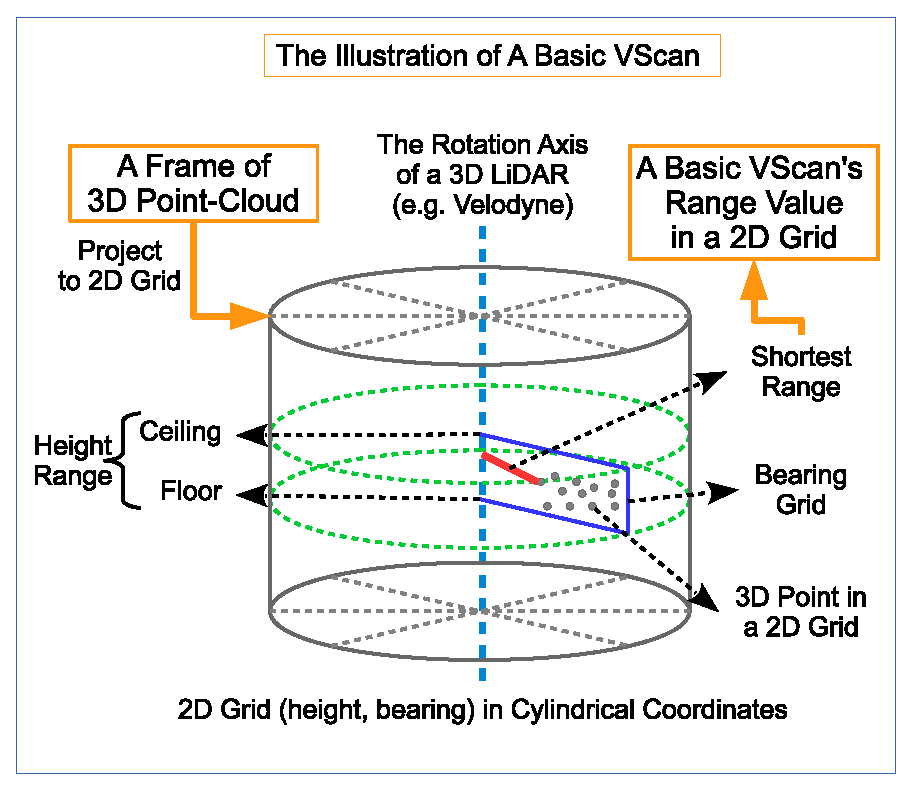
\includegraphics[width=\textwidth]{grid}
		\end{figure}
	\end{column}
\end{columns}

\begin{itemize}
\item Maecenas Vel Nisl Elit
\begin{itemize}
\item Suspendisse potenti. Fusce a est eget turpis rhoncus varius sed sed dui. Cras justo nibh, bibendum a cursus eget, consequat et dui. Maecenas vel nisl elit, sed dignissim dolor. 
\item In hac habitasse platea dictumst.
\end{itemize}

\item Viewpoint Matching Constraints
\begin{itemize}
\item Cum sociis natoque penatibus et magnis dis parturient montes, nascetur ridiculus mus. 
\item Proin in nisi diam.
\item Nam ultricies pellentesque nunc, ultrices volutpat nisl ultrices a.
\end{itemize}

\item Volutpat 
\begin{itemize}
\item Duis semper lorem eget dui dignissim porttitor.
\item Nulla facilisi. In ullamcorper lorem quis dolor.
\end{itemize}
\end{itemize}

\end{block}

%----------------------------------------------------------------------------------------

\end{column} % End of the first column

\begin{column}{.02\textwidth}\end{column} % Empty spacer column
 
\begin{column}{.48\textwidth} % The second column


%----------------------------------------------------------------------------------------
%	MATHEMATICAL SECTION
%----------------------------------------------------------------------------------------

\begin{block}{Algorithm Description}
	
	\begin{itemize}
		\item Maecenas Ultricies Feugiat Velit Non Mattis.
		\begin{itemize}
			\item Duis ante erat, bibendum nec tempus nec, interdum quis est. Nulla at mollis tortor. Phasellus quis leo dolor, aliquam laoreet orci $X$ Donec dapibus sagittis neque eu nec, interdum quis est. $Y_n, n=1,\cdots,N$ ndum nec tempus nec, interd
			\begin{align*}
			X \rightarrow r(X) & = \arg \max_{c} \Big\{ \max_n \big\{ \sum_{x_i \in X} \delta(x_i,Y_{n,c})\big\} \Big\} 
			\end{align*}
			\item Cras faucibus scelerisque cursus. Proin ut vestibulum augue. $\delta(x_i,Y_{n,c})$
		\end{itemize}
		\item Fusce tempus arcu id ligula varius dictum. Donec ut nisl dui, ac consectetur elit. In nec enim porta augue venenatis sollicitudin. Phasellus quis nunc neque. Suspendisse mauris diam, suscipit non gravida in, placerat id enim. Ut nec ipsum in lectus ultrices sagittis.
	\end{itemize}
	
\end{block}

%----------------------------------------------------------------------------------------
%	Experiment RESULTS
%----------------------------------------------------------------------------------------

\begin{block}{Experiment Results}

\begin{figure}
\includegraphics[width=0.8\linewidth]{placeholder.jpg}
\caption{Figure caption}
\end{figure}

\end{block}

%----------------------------------------------------------------------------------------
%	CONCLUSION
%----------------------------------------------------------------------------------------

\begin{block}{Conclusion}

\begin{itemize}
\item Opet volutpat ligula. Duis semper lorem eget dui dignissim porttitor. Nulla facilisi. In ullamcorper lorem quis dolor iaculis nec egestas enim ultricies. Cras ut mauris elit, ut lacinia dui. Proin in ante et libero hendrerit iaculis.
\item Nulla eu erat a urna laoreet auctor id a turpis. Nam mollis tristique neque eu luctus. Suspendisse rutrum congue nisi sed convallis. 
\item Aenean id neque dolor.
\item Opet volutpat ligula. Duis semper lorem eget dui dignissim porttitor. Nulla facilisi. In ullamcorper lorem quis dolor iaculis nec egestas enim ultricies. Cras ut mauris elit, ut lacinia dui. Proin in ante et libero hendrerit iaculis.
\end{itemize}

\end{block}

%----------------------------------------------------------------------------------------
%	REFERENCES
%----------------------------------------------------------------------------------------

\begin{block}{Main References}
        
\nocite{*} % Insert publications even if they are not cited in the poster
\small{\bibliographystyle{unsrt}
\bibliography{sample}}

\end{block}

%----------------------------------------------------------------------------------------
%	ACKNOWLEDGEMENTS
%----------------------------------------------------------------------------------------

\begin{block}{Acknowledgments}

\begin{itemize}
\item This research is supported by the Center of Innovation Program (Nagoya-COI: Mobility Society Leading to an Active and Joyful Life for Elderly) from Japan Science and Technology Agency.
\end{itemize}

\end{block}

%----------------------------------------------------------------------------------------
%	CONTACT INFORMATION
%----------------------------------------------------------------------------------------

\setbeamercolor{block title}{fg=black,bg=orange!70} % Change the block title color

\begin{block}{Contact Information}

\begin{itemize}
\item Web: \url{http://www.coi.nagoya-u.ac.jp}
\item Email: \url{mailto:alexanderhmw@gmail.com}{alexanderhmw@gmail.com}
\item Phone: +81-052-789-4841
\end{itemize}

\end{block}

%----------------------------------------------------------------------------------------

\end{column} % End of the second column

\begin{column}{.015\textwidth}\end{column} % Empty spacer column

\end{columns} % End of all the columns in the poster

\end{frame} % End of the enclosing frame

\end{document}